\section{Visto ieri: Sintesi caratteristiche di un s.d.}
Caratteristiche fondamentali per tutti i sistemi distribuiti:
\subsubsection{Gestione della memoria?}
\begin{itemize}
    \item \textbf{Non c'è memoria condivisa}
    \item Comunicazione via scambio messaggi
    \item Non c'è stato globale: ogni componente (nodo, processo) conosce solo il proprio stato e può sondare lo stato degli altri.
\end{itemize}

\subsubsection{Gestione dell'esecuzione?}
\begin{itemize}
    \item \textbf{Ogni componente è autonomo} => esecuzione concorrente
    \item Il coordinamento delle attività è importante per definire il comportamento di un sistema/applicazione costituita da più componenti
\end{itemize}

\subsubsection{Gestione del tempo (temporizzazione)?}
\begin{itemize}
    \item \textbf{Non c'è un clock globale}
    \item Non c'è possibilità di controllo/scheduling globale
    \item Solo coordinamento via scambio messaggi
\end{itemize}

\subsubsection{Tipi di fallimenti?}
\begin{itemize}
    \item \textbf{Fallimenti indipendenti} dei singoli nodi (independent failures)
    \item Non c'è fallimento globale
\end{itemize}

\section{Il modello Client-Server}
Il modello Client-Server è il modello di interazione tra un processo client e un processo server.
\begin{center}
    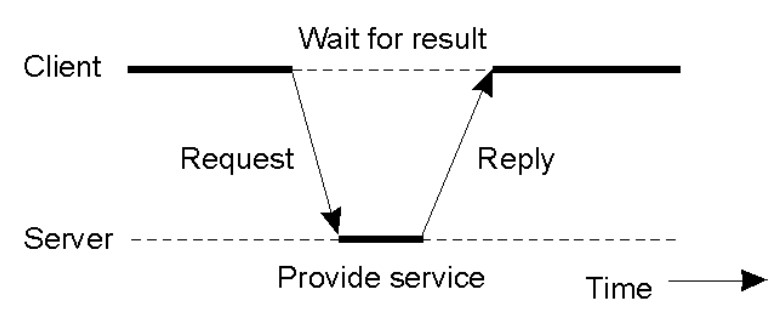
\includegraphics[width=0.5\textwidth]{img/modelloCS1.jpg}
\end{center}
C'è uno strato verticale e uno orizzontale(?)
\subsubsection{Configurazioni client/server}
\begin{itemize}
    \item Accesso a server multipli
    \item Accesso via proxy
\end{itemize}

\section{Caratteristiche problematiche di ogni sistema distribuito}
N.B.: (molto) probabile domanda d'esame.
\\Tutti i sistemi distribuiti vanno incontro a 4 problemi fondamentali che devono saper risolvere.
\\Vari step di risoluzione:
\begin{description}
    \item[Identificare la controparte]: fase di \textbf{naming}, dove assegnamo a  un identificativo che deve necessariamente essere \textbf{univoco}; 
    \item[Accedere alla controparte]: fase di \textbf{access point}, una \textit{reference} a cui possiamo fare riferimento;
    \item[Comunicazione 1]: fase di \textbf{protocol}, dove bisogna accordarsi su un formato condiviso di comunicazione (\textit{ricevere l'informazione});
    \item[Comunicazione 2]: questo è ancora un \textbf{open issue}, dove bisogna accordarsi su una convenzione di significato (\textit{capire l'informazione}).
\end{description}

\section{Trasparenza di distribuzione}
\begin{description}
    \item[Def.:] consiste nel nascondere dettagli agli utenti, che ignorano cosa succede e (più importante) non possono influenzare il servizio fornito. 
\end{description}
\begin{center}
    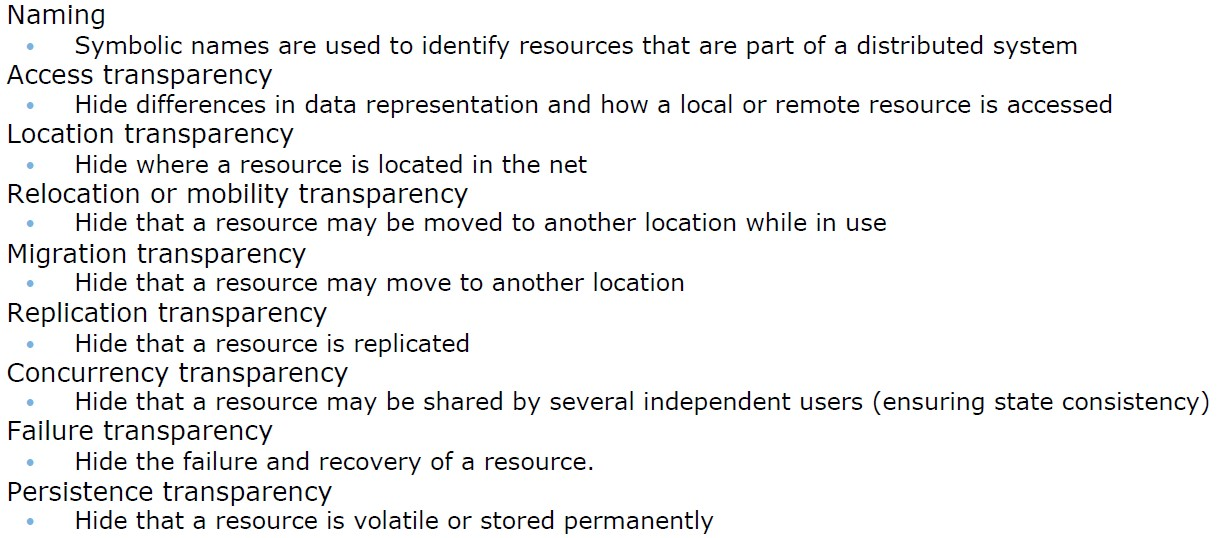
\includegraphics[width=0.75\textwidth]{img/trasparenza1.jpg}
\end{center}

% COSE

\section{Le basi dei sistemi distribuiti}
\subsection{Il concetto di protocollo}
Per poter capire le richieste e formulare le risposte i due processi devono concordare un \textbf{protocollo}.
\\I protocolli definiscono il \textbf{formato}, l'\textbf{ordine} di invio e di ricezione dei messaggi tra i dispositivi, il \textbf{tipo dei dati} e le \textbf{azioni} da eseguire quando si riceve un messaggio.
\\Le applicazioni su TCP/IP:
\begin{itemize}
    \item si scambiano \textbf{\textit{stream di byte}} di lunghezza infinita (il \textbf{meccanismo})
    \item che possono essere segmentati in \textbf{\textit{messaggi}} (la \textbf{politica}) definiti da un protocollo condiviso
\end{itemize}
Esempi di protocollo applicativi
\begin{itemize}
    \item HTTP - HyperText Transfer Protocol
    \item FTP - File Transfer Protocol
    \item SMTP - Simple Mail Transfer Protocol
\end{itemize}

\subsection{Elementi minimi per creare un'applicazione}
Definizione del protocollo di comunicazione.
\\Condivisione del protocollo tra gli attori dell'applicazione.
\\Un esempio in C:
\begin{center}
    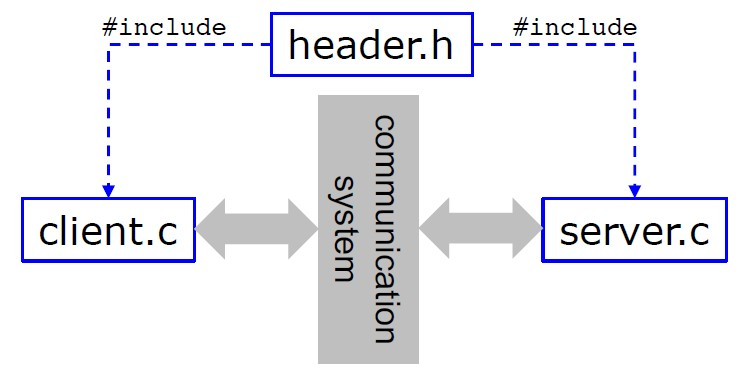
\includegraphics[width=0.75\textwidth]{img/esC_app1.jpg}
\end{center}
\subsubsection{Esempi: file server remoto}
\begin{center}
    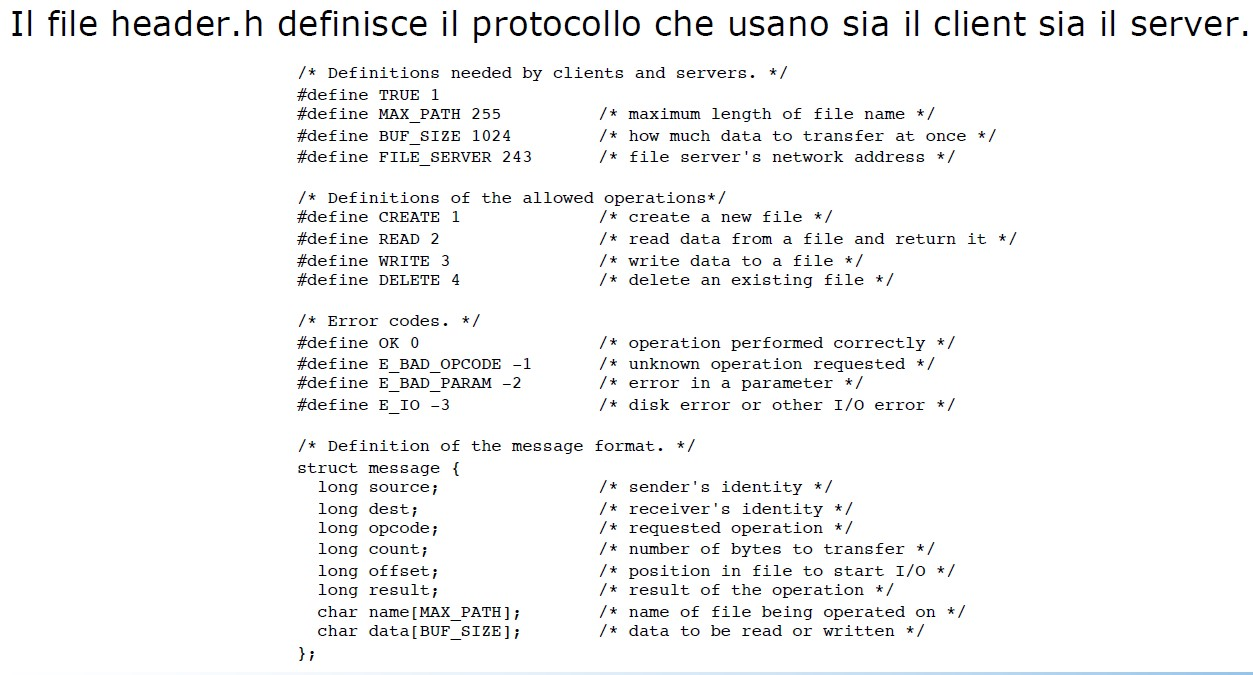
\includegraphics[width=0.75\textwidth]{img/es_serverRemoto1.jpg}
\end{center}
\begin{center}
    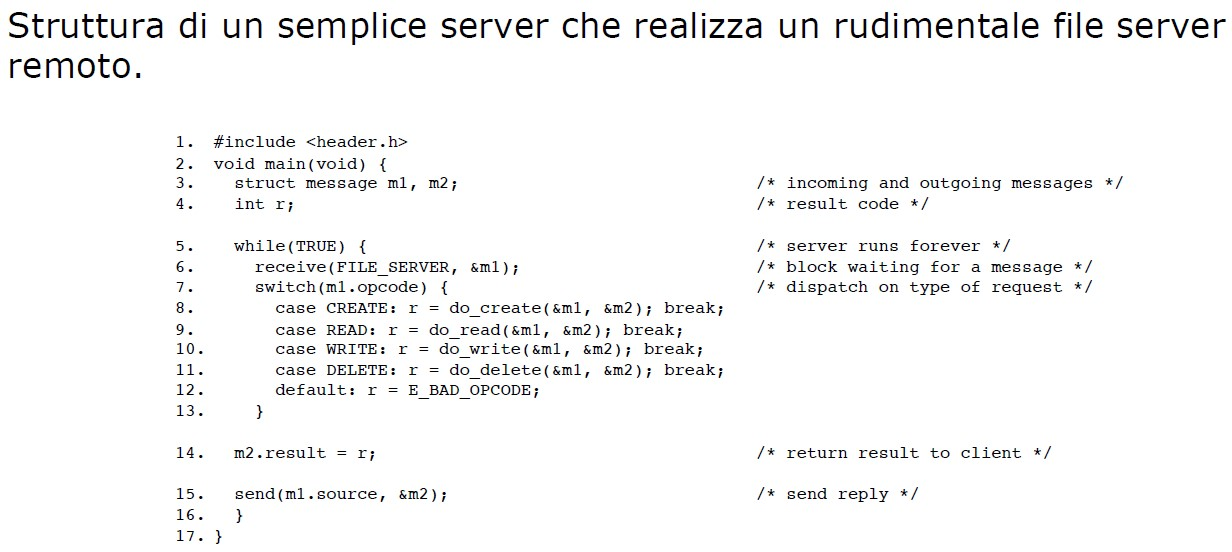
\includegraphics[width=0.75\textwidth]{img/es_serverRemoto2.jpg}
\end{center}
\begin{center}
    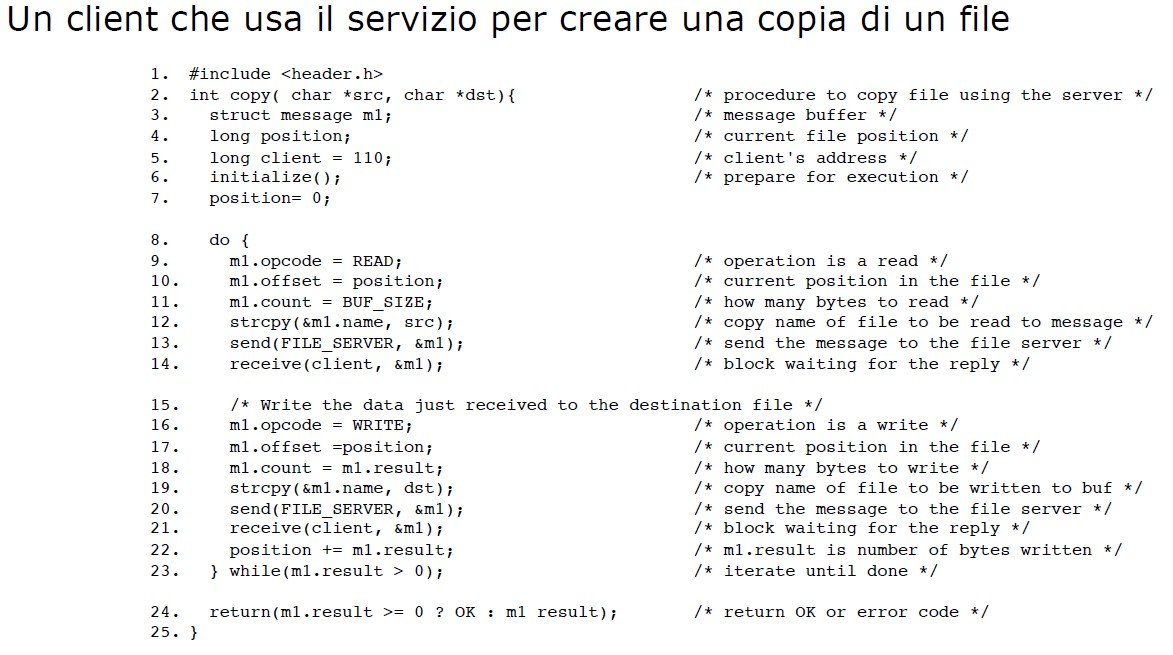
\includegraphics[width=0.75\textwidth]{img/es_serverRemoto3.jpg}
\end{center}

\chapter{Stream-oriented communication - Le socket}
\section{Contenuti sintetici}
Breve ripasso del modello ISO/OSI per TCP/IP
\\Identificazione dei processi
Indirizzi IP e Porte
L'interfaccia API per le socket
\\Le socket in Java
\\I modelli architetturali
\begin{itemize}
    \item Iterativo
    \item Concorrente mono processo
    \item Concorrente multi processo
\end{itemize}

\section{Modello ISO/OSI}

\section{Comunicazione fisica - layering}

\section{Network edge}
Chi è che si parla? I \textbf{processi}.

\section{Processi e programmi}
I programmi vengono eseguiti dai processi.
\begin{itemize}
    \item Programma = sequenza di istruzioni eseguibili dalla “macchina”
\end{itemize}
I processi sono entità gestite dal Sistema Operativo
\begin{itemize}
    \item Processo = area di memoria RAM per effettuare le operazioni e memorizzare i dati + registro che ricorda la prossima istruzione da eseguire + canali di comunicazione
\end{itemize}
Ogni processo comunica attraverso canali.
\begin{itemize}
    \item Un canale gestisce flussi di dati in ingresso e in uscita (dati in formato binario o testuale)
    \item Per esempio lo schermo, la tastiera e la rete sono “canali”
    \item Dall'esterno ogni canale è identificato da un numero intero detto “porta”
\end{itemize}
Le socket sono particolari canali per la comunicazione tra processi che non condividono memoria (per esempio perché risiedono su macchine diverse).
\\Per potersi connettere o inviare dati ad un processo A, un processo B deve conoscere la macchina (host) che esegue A e la porta cui A è connesso (wellknown port).

\section{I servizi di trasporto Internet}
\begin{center}
    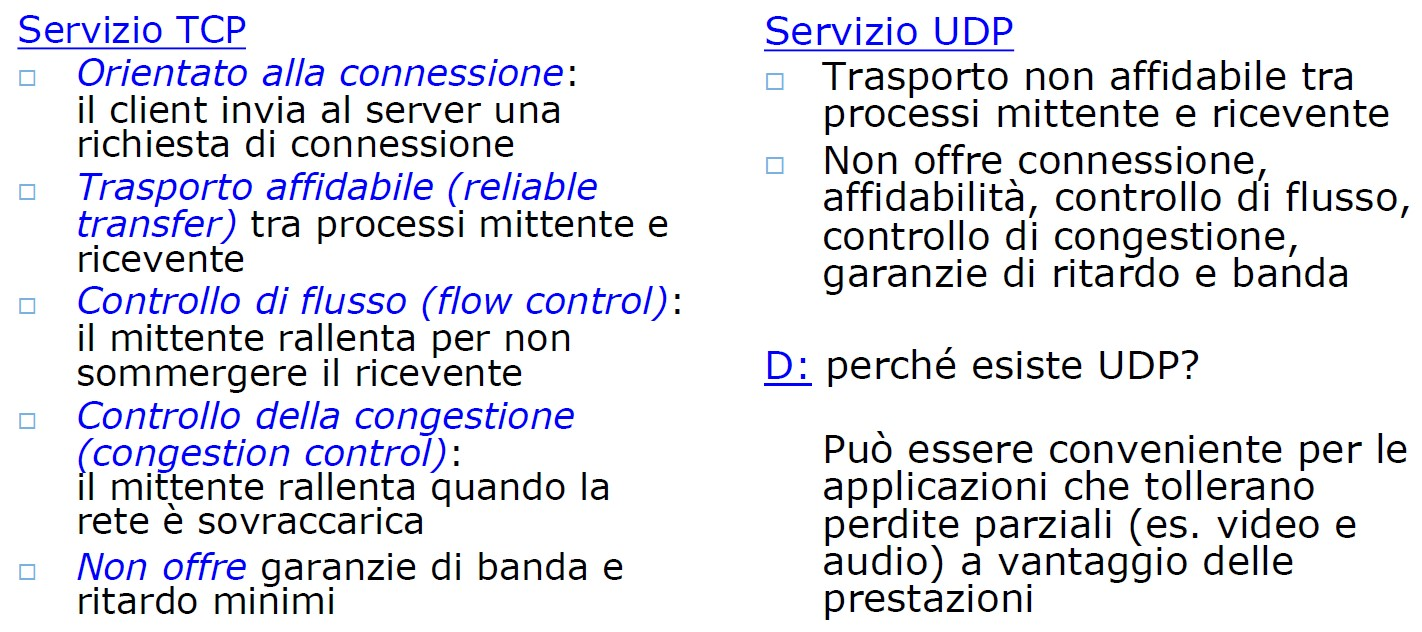
\includegraphics[width=0.75\textwidth]{img/servizi_trasporto_internet1.jpg}
\end{center}

\section{Politiche dei servizi TCP/UDP}
\subsubsection{Servizio UDP:}
\begin{itemize}
    \item Scompone il flusso di byte in segmenti
    \item Li invia, uno per volta, ai servizi network
\end{itemize}
\subsubsection{Servizio TCP:}
\begin{itemize}
    \item Scompone e invia come UDP
    \item Ogni segmento viene numerato per garantire:
    \\• Riordinamento dei segmenti arrivati
    \\• Controllo delle duplicazioni (scarto i segmenti con ugual numero d'ordine)
    \\• Controllo delle perdite (rinvio i segmenti mancanti)
    \item Per progettare e realizzare sistemi distribuiti
    \\• NON è necessario conoscere il funzionamento (information hiding) dei processi
    \\• Ciò che importa è lo scambio dati (stream di byte) tra i processi
\end{itemize}

\section{Socket: funzionamento di base}
\subsubsection{TCP}
\begin{itemize}
    \item Utilizza variabili e buffer per realizzare il trasferimento bidirezionale di flussi di bytes (“pipe”) tra processi
    \item Prevede ruoli client/server durante la connessione
    \item NON prevede ruoli client/server per la comunicazione
    \item Utilizza i servizi dello strato IP per l'invio dei flussi di bytes
\end{itemize}
\subsubsection{API: Application Programming Interface}
\begin{itemize}
    \item Definisce l'interfaccia tra applicazione e strato di trasporto
\end{itemize}
\subsubsection{Socket: API per accedere a TCP e UDP}
\begin{itemize}
    \item Due processi (applicazione nel modello client server) comunicano inviando/leggendo dati in/da socket
\end{itemize}

\section{Aspetti critici}
Gestione del ciclo di vita di client e server
• Attivazione/terminazione del cliente e del server
(es. Manuale o gestita da un middleware)
¨ Identificazione e accesso al server
• Informazioni che deve conoscere il cliente per accedere al server
¨ Comunicazione tra cliente e server
• Le primitive disponibili e le modalità per la comunicazione
(es. TCP/IP: Stream di dati inviati con send/receive)
¨ Ripartizione dei compiti tra client e server
• Dipende dal tipo di applicazione
(es. controllo: una banca gestisce tutto lato server)
• Influenza la prestazioni in relazione al carico (numero di clienti)

\section{Identificare il server}
Come fa il client a conoscere l'indirizzo del server?
¨ Alternative:
• inserire nel codice del client l'indirizzo del server espresso come costante
(es. il client di un servizio bancario)
• chiedere all'utente l'indirizzo (es. web browser)
• utilizzare un name server o un repository da cui il client può acquisire le
informazioni necessarie
(es. Domain Name Service - DNS - per tradurre nomi simbolici)
• adottare un protocollo diverso per l'individuazione del server
(es. broadcast per DHCP)

\section{Problemi fondamentali e TCP/IP}
Come sono trattate le 4 problematiche fondamentali dei sistemi distribuiti con TCP e IP?
\begin{description}
    \item[Identifico la controparte (naming):]
    \item[] Low level identification: the name of hosts and protocols
    \item[Accedo alla controparte (access point):]
    \item[] Use of the IP address (host:port) to access a process
    \item[Comunicazione 1 (protocollo):]
    \item[] Stream of bytes
    \item[Comunicazione 2 (sintassi e semantica):]
    \item[] Application protocols with predefined semantics (http, smtp)
    \item[What level of transparency?] Very low: the programmer/user need to
    \item[] - know network addresses
    \item[] - parse bytes to get the content (message)
\end{description}

\textbf{IMPORTANTE}: TCP si può usare per qualsiasi tipo di comunicazione? Perché non c'è semantica. Quindi il punto di Comunicazione 2 non c'è. Questa potrebbe essere una domanda dell'esame.

\section{Comunicazione via socket}
La comunicazione TCP/IP avviene attraverso flussi di byte (byte stream), dopo una connessione esplicita, tramite normali system call read/write.
\\Read e write:
\begin{itemize}
    \item Sono sospensive (bloccano il processo finché il sistema operativo non ha effettuato la lettura/scrittura)
    \item Utilizzano un buffer per garantire flessibilità (es: la read definisce un buffer per leggere N caratteri, ma potrebbe ritornare avendone letti solo k<N)
\end{itemize}
\begin{center}
    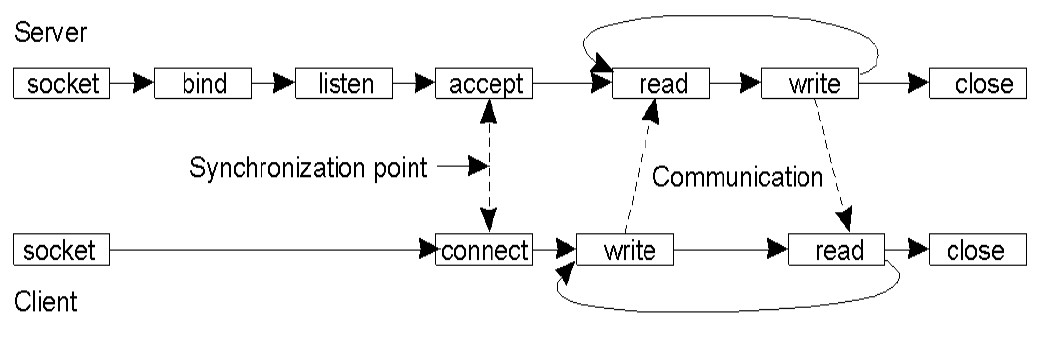
\includegraphics[width=0.75\textwidth]{img/socket_comunicazione1.jpg}
\end{center}

\section{API socket system calls (Berkeley)}
Many calls are provided to access TCP and UDP services.
\\The most relevant ones are in the table below:
\begin{center}
    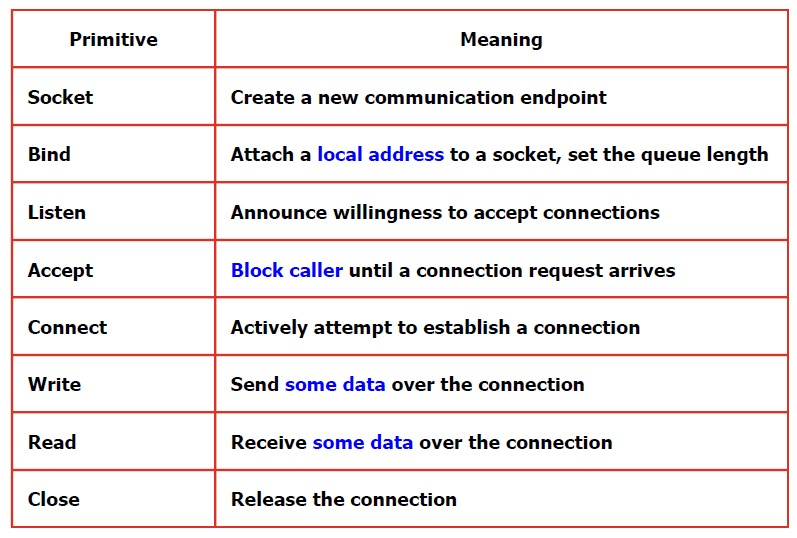
\includegraphics[width=0.75\textwidth]{img/berkeley1.jpg}
\end{center}